\documentclass[a4paper]{article}

\usepackage[czech]{babel} %https://github.com/michal-h21/biblatex-iso690
\usepackage[
   backend=biber      % if we want unicode 
  ,style=iso-numeric % or iso-numeric for numeric citation method          
  ,babel=other        % to support multiple languages in bibliography
  ,sortlocale=cs_CZ   % locale of main language, it is for sorting
  ,bibencoding=UTF8   % this is necessary only if bibliography file is in different encoding than main document
]{biblatex}

\usepackage[utf8]{inputenc}
\usepackage{fancyhdr}
\usepackage{amsmath}
\usepackage{amssymb}
\usepackage[left=2cm,right=2cm,top=2.5cm,bottom=2.5cm]{geometry}
\usepackage{graphicx}
\usepackage{pdfpages}
\usepackage{url}

\usepackage{siunitx}
\sisetup{locale = DE}  %, separate-uncertainty = true    kdybych chtel +/-

\usepackage{float}
\newfloat{graph}{htbp}{grp}
\floatname{graph}{Graf}
\newfloat{tabulka}{htbp}{tbl}
\floatname{tabulka}{Tabulka}

\renewcommand{\thefootnote}{\roman{footnote}}

\pagestyle{fancy}
\lhead{Praktikum II - (19) Měření s torzním magnetometrem}
\rhead{Vladislav Wohlrath}
\author{Vladislav Wohlrath}

\bibliography{source}

\begin{document}

\begin{titlepage}
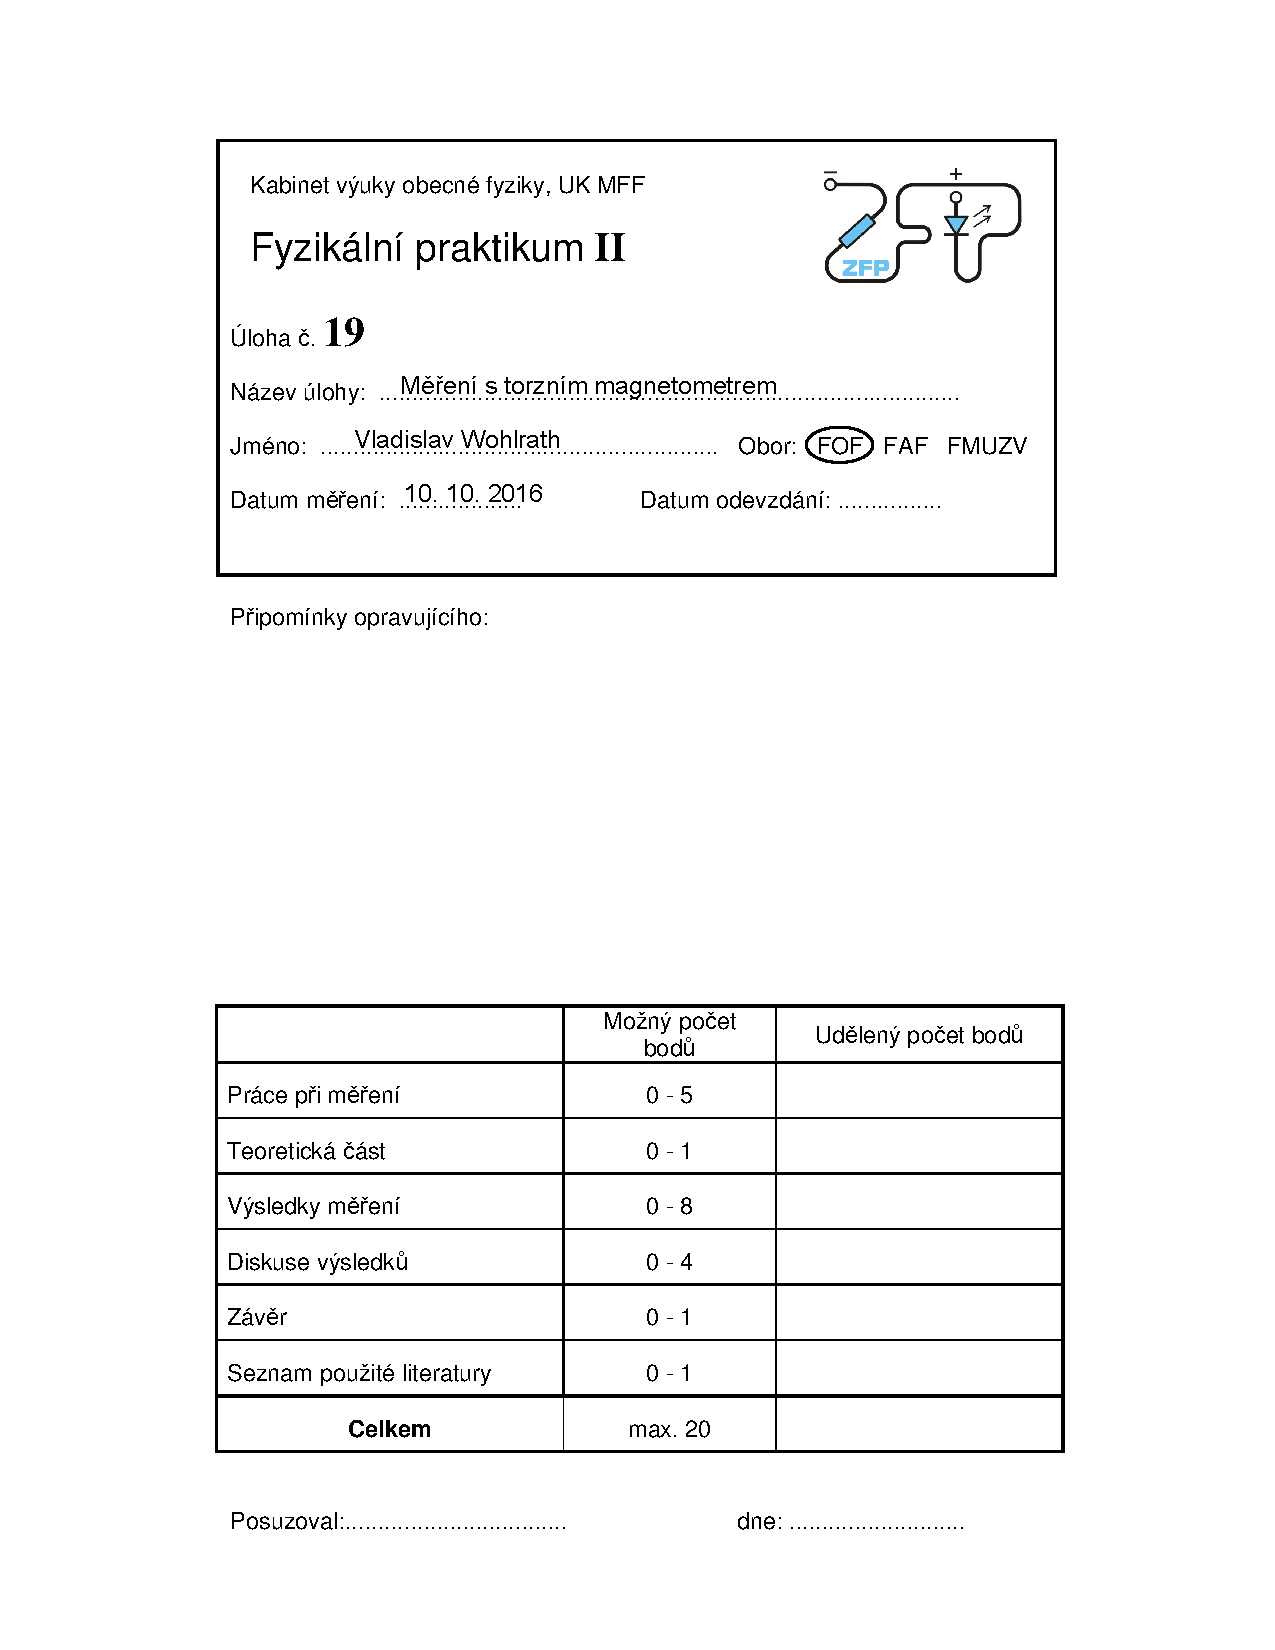
\includepdf[pages={1}]{./graficos/219-tit.pdf}
\end{titlepage}

\section*{Pracovní úkoly}
\begin{enumerate}
\item Změřte závislost výchylky magnetometru na proudu protékajícím cívkou. Měření proveďte pro obě cívky a různé počty závitů (\num{5} a \num{10}).
\item Výsledky měření znázorněte graficky.
\item Diskutujte výsledky měření z hlediska platnosti Biot-Savartova zákona.
\item Změřte direkční moment vlákna metodou torzních kmitů.
\item Určete magnetický moment magnetu užívaného při měření (v Coulombových i Ampérových jednotkách). 
\end{enumerate}

%Teoretická část
\section*{Teoretická část}

%Výsledky měření
\section*{Výsledky měření}


%Diskuze výsledků
\section*{Diskuze}

%Závěr
\section*{Závěr}
Změřili jsme závislost výchylky magnetometru na proudu procházejícím cívkou pro dvě různé cívky a různé počty závitů.
Naměřené hodnoty jsou uvedeny v tabulce \ref{tab:tabmain} a zaneseny do grafu \ref{graf:grafmain}.
Do grafu je též vynesena teoretická závislost vyplývající z Biotova-Savartova zákona.
Hodnoty se dobře shodují, takže Biotův-Savartův zákon zůstává v platnosti.

Dále jsme metodou torzních kmitů změřili direkční moment vlákna v magnetometru $D=\num{6.6(2)}\cdot \SI{e-4}{\newton\metre\per\radian}$.

Z naměřené závislosti jsme určili Coulombův magnetický moment $p = \num{3.8(2)} \cdot \SI{e-7}{\weber \meter}$ nebo též Ampérův magnetický moment $m = \SI{0.30(2)}{\ampere\metre\squared}$.


\printbibliography[title={Seznam použité literatury}]

\end{document}